\documentclass[a4paper,10pt]{jsarticle}

% レイアウト
\setlength{\textwidth}{\fullwidth}
\setlength{\textheight}{39\baselineskip}
\addtolength{\textheight}{\topskip}
\setlength{\voffset}{-0.5in}
\setlength{\headsep}{0.3in}
\pagestyle{myheadings}

% パッケージ
\usepackage[dvipdfmx]{graphicx}
\usepackage{amsmath,amssymb,epsfig}
\usepackage{bm}
\usepackage{ascmac}
\usepackage{pifont}
\usepackage{multirow}
\usepackage{enumerate}
\usepackage{cases}
\usepackage{type1cm}
\usepackage{cancel}
\usepackage{url}
\usepackage{color}
\usepackage{listings,jlisting}
% 大きな中括弧
\usepackage{cases}

% 定義
\DeclareMathOperator*{\argmin}{arg\,min}
\DeclareMathOperator*{\argmax}{arg\,max}
\def\vec#1{\mbox{\boldmath$#1$}}
\def\R{{\Bbb R}}

% カウンタの設定
\setcounter{section}{0}
\setcounter{subsection}{0}
\setcounter{subsubsection}{0}
\setcounter{equation}{0}

% キャプションの図をFigに変更
\renewcommand{\figurename}{Fig.}
\renewcommand{\tablename}{Tab.}

% 式番号を式(章番号.番号)に
\makeatletter
\renewcommand{\theequation}{\arabic{section}.\arabic{equation}}
\@addtoreset{equation}{section}
\makeatother

% プログラムに色をつける
\usepackage{color}

\definecolor{codegreen}{rgb}{0,0.6,0}
\definecolor{codegray}{rgb}{0.5,0.5,0.5}
\definecolor{codepurple}{rgb}{0.58,0,0.82}
\definecolor{backcolour}{rgb}{0.95,0.95,0.92}

\lstdefinestyle{mystyle}{
    backgroundcolor=\color{backcolour},
    commentstyle=\color{codegreen},
    keywordstyle=\color{magenta},
    numberstyle=\tiny\color{codegray},
    stringstyle=\color{codepurple},
    basicstyle=\footnotesize,
    breakatwhitespace=false,
    breaklines=true,
    captionpos=b,
    keepspaces=true,
    numbers=left,
    numbersep=5pt,
    showspaces=false,
    showstringspaces=false,
    showtabs=false,
    tabsize=2
}

\lstset{style=mystyle}

% 表紙
\title{知能システム学特論レポート}
\author{
(DL2班)Caffe on Ubuntu\\
}
\date{2015年\ 7月\ 13日}

% ドキュメントの開始
\begin{document}
\maketitle
\section{報告者}
\begin{list}{}{}
 \item 15344203\hspace{0.5cm} 有田 裕太
 \item 15344206\hspace{0.5cm} 緒形 裕太
 \item 15344209\hspace{0.5cm} 株丹 亮
 \item 12104125\hspace{0.5cm} 宮本 和
\end{list}

\section{進行状況}

\begin{itemize}
\item 畳み込みネットワークと正規化層の理論について
\item データセットの作成準備
\end{itemize}

\section{理論研究}

\subsection{畳込み層}

% 実用的な畳込みネットでは,グレースケールの画像1枚に対してではなく,多チャネルの画像に対し,複数個のフィルタを並行して畳込む演算を行う.チャネルの画像とは各画素が複数の値を持つ画像であり,チャネル数がKの画像の各画素はK個の値を持つ.例えば,グレースケールの画像では$K = 1$,RGBの3色からなるカラー画像では$K = 3$となる.畳込みネットの中間層では,さらにそれ以上のチャネル数の画像を扱う.以下では,画像の縦横の画素数が $W \times W$でチャネル数が K のとき,画像のサイズを$W \times W \times K$と書く.

% 濃淡地を各画素に格納したグレースケールの画像を考える.
% 画像サイズを$W\times W$画素とし,画素をインデックス$(i,j)(i = 0,\cdots,W-1, j = 0,\cdots,W-1)$で表す.
% これまでインデックスは1から開始していたが,画像(及びそれに類するもの)を扱う場合はインデックスを0から始めることとする.
% 画素$(i,j)$の画素値を$x_{ij}$と書き,負の値を含む実数値をとるとする.
% そして,この画像に適用する $H\times H$画素のフィルタ
% (サイズの小さい画像)を考える.このフィルタのインデックス$(p,q)(p=0,\cdots,H-1, q=0,\cdots,H-1)$で表し,画素値を$h_{pq}$と書く.

% \begin{figure}[t]
%  \centering
%  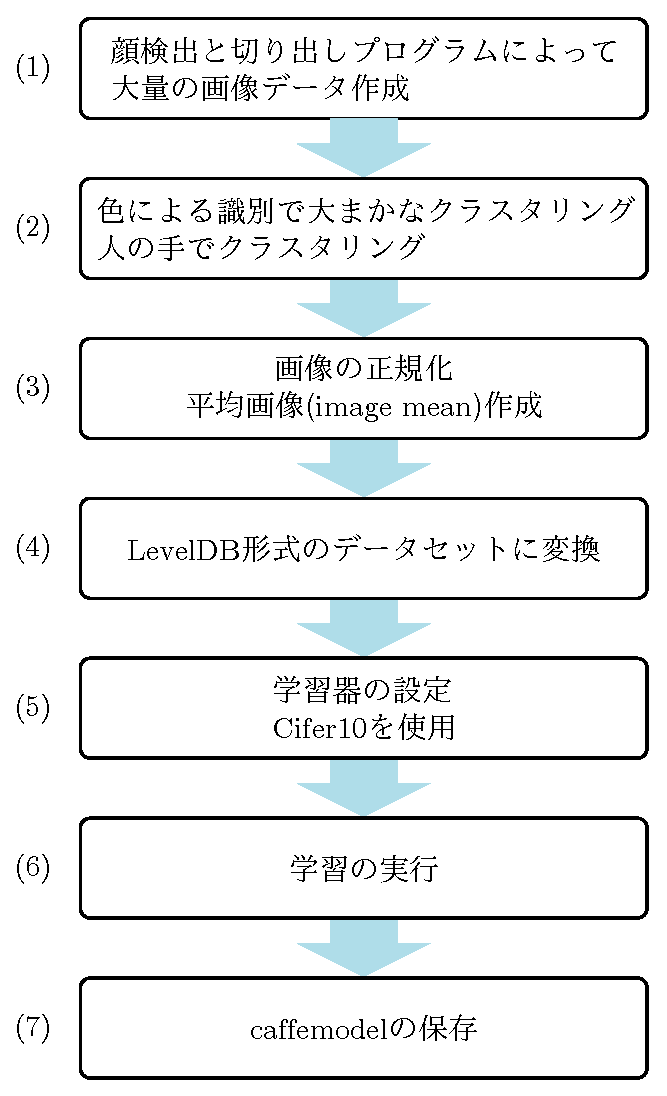
\includegraphics[scale=0.4]{fig/eps/learning_flow.eps}
%   \caption{畳み込み層の概要}
%   \label{fig:畳み込み層の概要}
% \end{figure}

% 図1を用いて畳込み層での計算を説明する.この畳込み層は直前の層からKチャネルの画像 $x_{ijk} (k = 0,...,K − 1)$ を受け取り,これに$ M = 3 $種類のフィルタ $h_{pqkm} (m = 0,...,M − 1)$ を適用している.各フィルタ ($m = 0, 1, 2$) は通常,入力と同じチャネル数$K$を持ち(サイズを $H \times H \times K $とする),図1のようにフィルタごとに計算は並行に実行される.計算の中身は,そのフィルタの各チャネルごとに,これも並行に画像とフィルタの畳込みを行った後,結果を画素ごとに全チャネルにわたって加算する.

% \begin{equation}
%   u_{ijm} = \sum_{p=0}^{K-1} \sum_{q=0}^{H-1} \sum_{q=0}^{H-1} z_{i+p,j+q,k}^{(l-1)} h_{pqkm}+b_{ijm}
% \end{equation}
% 入力画像のチャネル数によらず,1つのフィルタからの出力は常に1チャネルになる.

\subsection{単一チャネルの正規化}
単一チャネルの画像$x_{ij}$に対し,プーリングと同様,画素$(i,j)$を中心と
する$H\times H$の正方領域$P_{ij}$を考える.減算正規化とは,入力画像の各
画素濃淡から,$P_{ij}$に含まれる画素の濃淡の平均,つまり
$\bar{x}_{ij}= \sum_{(p,q)\in{P_{ij}}}^{} x_{i+p,j+q}$を差し引く.
\begin{equation}
 z_{ij} = x_{ij}-\bar{x}_{ij} 
\end{equation}
ここで差し引く$\bar{x}_{ij}$には,重み付き平均
\begin{equation}
 \bar{x}_{ij}=\sum_{(p,q)\in{P_{ij}}} w_{pq}x_{i+p,j+q}
\end{equation}
を使う場合もある.その場合$w_{pq}$は
\begin{equation}
  \sum_{(p,q)\in{P_{ij}}}^{} w_{pq} = \sum_{q=0}^{H-1} \sum_{q=0}^{H-1} w_{pq}=1
\end{equation}
であり,領域の中央で最大値をとり,周辺部へ向けて低下するようなものとする.
領域の中央部をより重視し,周辺部の相対的な影響を少なくるためである.

同じ領域内で,さらに画素値の分散を抑える操作が除算正規化である.$P_{ij}$
内の画素値の分散は
\begin{equation}
 \omega^2_{ij}=\sum_{(p,q)\in{P_{ij}}}^{} w_{pq}(x_{i+p,j+q}-\bar{x}_{ij})^2
\end{equation}
となるが,減算正規化を施した入力画像をこの標準偏差で割る.
\begin{equation}
 z_{ij}=\frac{x_{ij}-\bar{x}_{ij}}{\omega_{ij}} 
\end{equation}
この計算をそのまま行うと,濃淡変化が少ない局所領域ほど濃淡変化が増幅され,
ノイズが強調される.そこで,入力画像のコントラストが大きい部分にのみ適用
するために,ある定数$c$を設定し,濃淡の標準偏差がこれを下回る
($\omega_{ij}<c$)で除算する
\begin{equation}
 z_{ij}=\frac{x_{ij}-\bar{x}_{ij}}{max(\omega_{ij}<c)}
\end{equation}
や,同様の効果が$\omega_{ij}$に応じて連続的に変化する
\begin{equation}
 z_{ij}=\frac{x_{ij}-\bar{x}_{ij}}{\sqrt{\omega_{ij}+c}} 
\end{equation}
を使う.減算正規化および式\ref{}による除算正規化の計算例を図
\ref{}に示す.
これらの正規化の結果,画像の画素値は負の値をとり得るため,画素値の最大値
と最小値が[0,255]の範囲に収まるように画素値を線形変換している.

\subsection{プーリング}
% プーリング層は通常,畳み込み層の直後に設置される.プーリング層は畳み込み層で抽出された特徴の位置感度を低下させる働きがあり,対象とする特徴量の画像内での位置が若干変化した場合においても,プーリング層の出力が不変になるようにする.

% プーリング層での計算は次のようにして行う.サイズ$W \times W \times K$の入力画像上で画素$(i,j)$を中心とする$H\times H$の正方領域とり,この中に含まれる画素の集合を$P_{ij}$で表す.$P_{ij}$内の画素についてチャネル$k$ごとに独立に,$H^2$個ある画素値を使って1つの画素値$u_{ijk}$を求める.これにはいくつかの方法があり,最大プーリング(max pooling)は,$H^{2}$個の画素値の最大値を選ぶ.
% \begin{eqnarray}
%  u_{ijk} = \max_{(p,q) \in P_{ij}} z_{pqk}
% \end{eqnarray}
% また,平均プーリング(average pooling)はそれらの平均値を計算する.
% \begin{eqnarray}
%  u_{ijk} = \frac{1}{H^{2}}\sum_{(p,q) \in P_{ij}} z_{pq}
% \end{eqnarray}
% 通常は,プーリング層の出力のチャネル数は入力画像のチャネル数と一致する.
% これらのプーリングを含む一般性を持った表記として,次のLpプーリング(Lp pooling)がある.
% \begin{eqnarray}
%  u_{ijk} = \left(\frac{1}{H^{2}}\sum_{(p,q) \in P_{ij}}z^{P}_{pqk}\right)^{\frac{1}{P}}
% \end{eqnarray}
% $P=1$で平均プーリング,$P=\infty$で最大プーリングが表現できる.なお,画像認識では最大プーリングが良く用いられている.

% プーリング層では2以上のストライドを設定することが普通である.プーリング層では結合の重みは固定されており,学習によって変化するパラメータはない.
% \begin{figure}[bt]
%  \centering
%  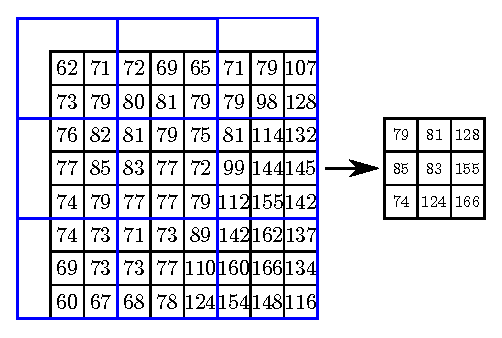
\includegraphics[scale = 1]{fig/eps/pooling.eps}
%  \caption{プーリングの例.プーリングサイズ$3\times 3$,ストライド$s=3$,ゼロパディングで最大プーリングを行った場合}
% \end{figure}

\section{プログラミング}
\subsection{画像を学習させて分類器を作るまでの流れ}
データセットを作成し,学習を行ってモデルを作成するまでの流れをFig.~\ref{fig:モデルを作成するまでの流れ}に示す.
Fig.~\ref{fig:モデルを作成するまでの流れ}より(1)の大量の写真データまたは動画からの切り出しに関しては
\begin{figure}[tb]
  \begin{center}
    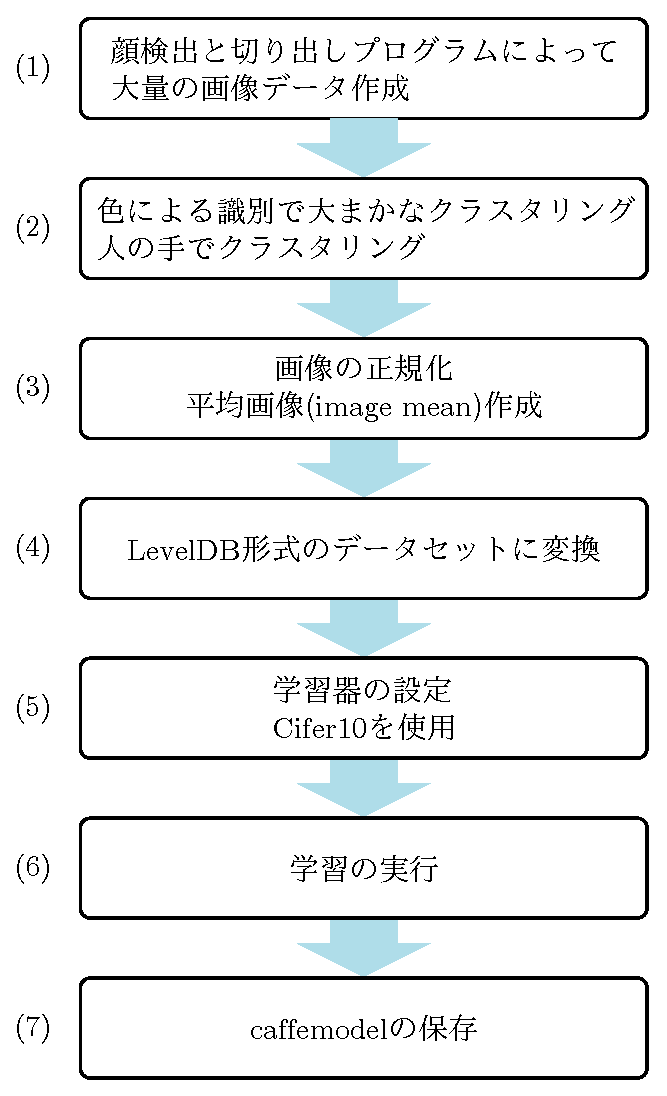
\includegraphics[clip,width=6cm]{fig/eps/learning_flow.eps}
  \end{center}
  \caption{モデルを作成するまでの流れ}
  \label{fig:モデルを作成するまでの流れ}
\end{figure}


\section{今後の課題}
\begin{itemize}
 \item 理論研究を進める.
 \item データセットの作成,学習の実行
\end{itemize}

\end{document}